% DO NOT COMPILE THIS FILE DIRECTLY!
% This is included by the other .tex files.
\begin{frame}[t,plain]
\titlepage
\end{frame}

\begin{frame}{Outline Day 1}
    \tableofcontents
\end{frame}


\section{Introduction (C1)}
\begin{frame}{What is Android?}
\begin{itemize}
\item Android represents an exciting new
opportunity to write innovative applications for
mobile devices.
\item Android is an \textbf{open-source software stack} that
includes the \textbf{operating system}, \textbf{middleware}, and \textbf{key mobile applications} along
with a set of \textbf{API libraries} for writing mobile applications that can shape the
look, feel, and function of mobile handsets.
\end{itemize}
\end{frame}

\begin{frame}{Android devices}
Small, stylish, and versatile, modern mobile
devices have become powerful tools that
incorporate \textbf{cameras, media players, GPS
systems, touchscreens} and other \textbf{sensors}.\\

\includegraphics[height=1.5cm]{images/motorola}\hfill

\includegraphics[height=1.5cm]{images/se}\hfill

\includegraphics[height=1.5cm]{images/htc}\\

\includegraphics[width=3cm]{images/samsung}\hfill

\includegraphics[width=3cm]{images/lg}\hfill

\includegraphics[width=3cm]{images/zte}\\
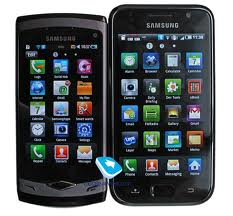
\includegraphics[width=2cm]{images/phone}\hfill
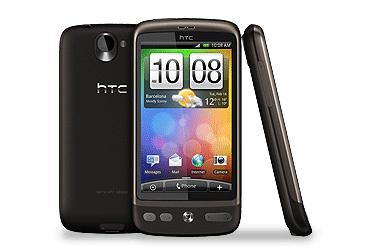
\includegraphics[width=2cm]{images/phone1}\hfill
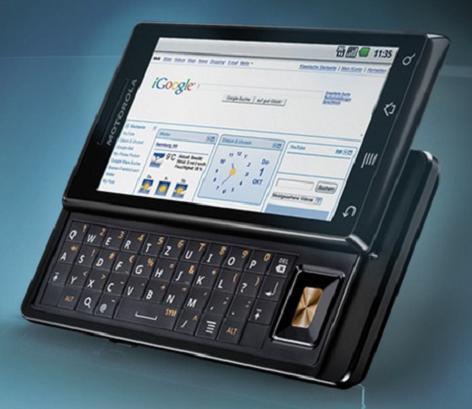
\includegraphics[width=2cm]{images/slide}\hfill
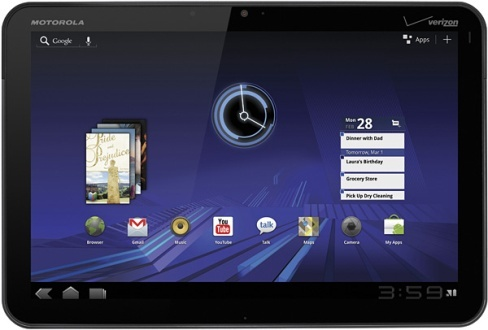
\includegraphics[width=2cm]{images/tablet}\hfill
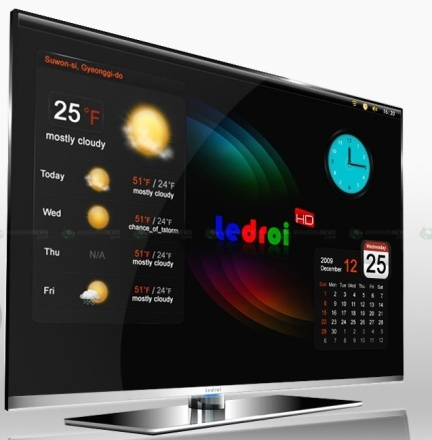
\includegraphics[width=2cm]{images/tv}
\end{frame}

\begin{frame}{Resourses}
\begin{itemize}
    \item Android Developers
        \begin{itemize}
          \item \href{http://developer.android.com}{http://developer.android.com}
        \end{itemize}
    \item Download SDK
        \begin{itemize}
          \item \href{http://developer.android.com/sdk/index.html}{http://developer.android.com/sdk/index.html}
        \end{itemize}
    \item Android Market
        \begin{itemize}
          \item \href{http://market.android.com}{http://market.android.com}
          \item \href{https://market.android.com/publish/}{https://market.android.com/publish/}
        \end{itemize}
\end{itemize}
\end{frame}

\begin{frame}{Application development}
\begin{itemize}
  \item Android native application
  \begin{itemize}
    \item Build using the Android SDK and Java programming
language
  \end{itemize}
  \item Browser application
  \begin{itemize}
    \item Android has browser with full web capabilities
    \item All standard web application
    \item jQuery
  \end{itemize}
\end{itemize}
\end{frame}

\section{Android Overview (C2)}

\begin{frame}{Android Architecture}
\begin{center}
    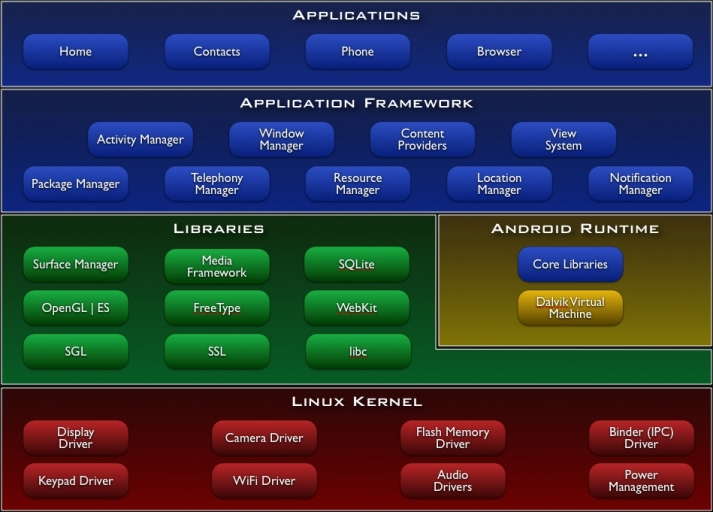
\includegraphics[scale=0.36]{images/architecture}
\end{center}
\end{frame}

\begin{frame}{Android Application Model}
\begin{center}
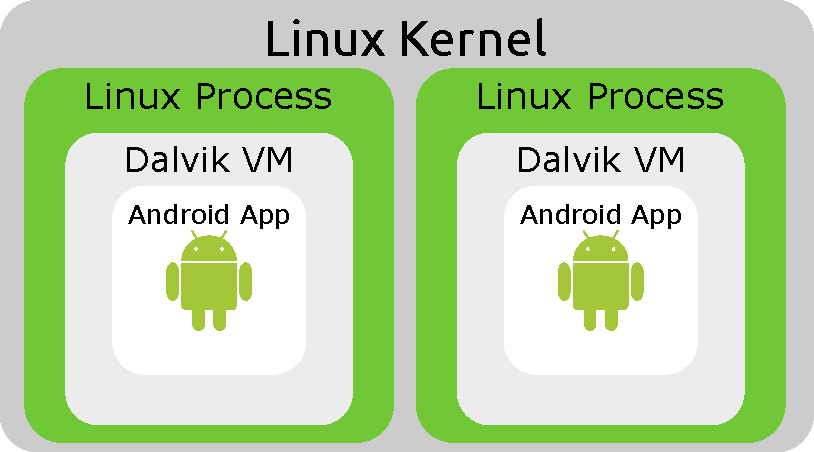
\includegraphics[scale=0.6]{images/application_model}
\end{center}
\end{frame}

\begin{frame}{The Dalvik Virtual Machine}
\begin{itemize}
  \item Custom VM
  \item Ensures that multiple instances run efficiently
on a single device
  \item Uses the device's underlying Linux kernel to
handle low-level functionality
    \begin{itemize}
        \item The Dalvik VM executes Dalvik executable files
        Format optimized to ensure minimal memory
        footprint
        \item Creates .dex executables
    \end{itemize}
\end{itemize}
\end{frame}

\begin{frame}{Responsiveness (ANR)}{Application not responding}
\begin{center}
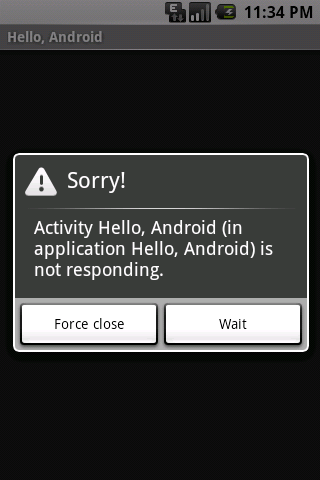
\includegraphics[scale=0.3]{images/anr}
\end{center}
\end{frame}

\begin{frame}{Platform Components}
\begin{itemize}
  \item Activities
  \begin{itemize}
    \item Your application’s presentation layer
   \end{itemize}
  \item Services
  \begin{itemize}
  \item The invisible workers of your application
  \end{itemize}
  \item Content Providers
  \begin{itemize}
  \item Shareable data stores
  \end{itemize}
  \item Intents
  \begin{itemize}
  \item An inter-application message-passing framework
  \end{itemize}
  \item Broadcast Receivers
  \begin{itemize}
  \item Intent broadcast consumers
  \end{itemize}
  \item Widgets
  \begin{itemize} 
  \item Visual application components that can be added to the home
  screen
  \end{itemize}
  \item Notifications
  \begin{itemize}
  \item A user notification framework
  \end{itemize}
\end{itemize}
\end{frame}

\begin{frame}{The Activity Life Cycle}
\begin{center}
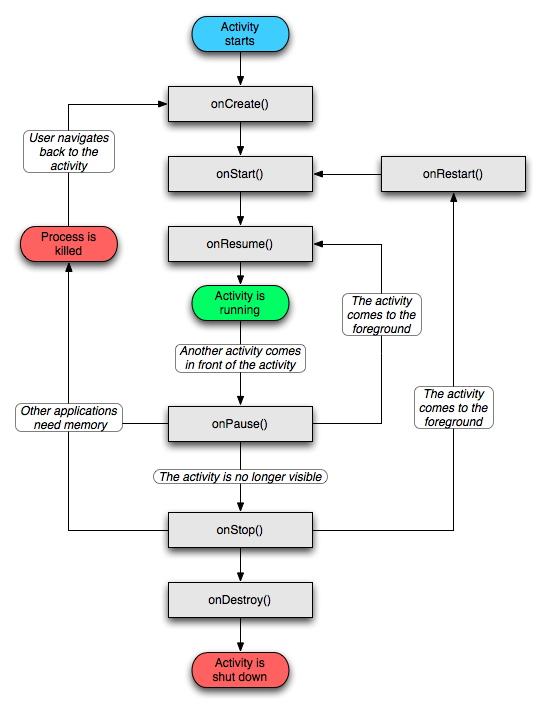
\includegraphics[scale=0.25]{images/life_cycle}
\end{center}
\end{frame}

\section{Steps in Android Application Development (C3)}

\begin{frame}{Development Environment}
\begin{itemize}
  \item Preparing Your Development Computer
  \begin{itemize}
  \item JDK (Java Development Kit)
  \item Eclipse
  \end{itemize}
  \item Downloading the SDK Starter Package
  \item Installing the ADT Plugin for Eclipse
  \item Adding Platforms and Other Components
  \item Exploring the SDK (Optional)
\end{itemize}
\end{frame}

\begin{frame}{Hello world application}

\end{frame}

\begin{frame}{Toolchains}
\begin{itemize}
  \item Android SDK
  \begin{itemize}
  \item Emulator
  \end{itemize}
  \item DDMS
  \item Hierarchy Viewer
  \item Trace View
  \item Nine Patch Editor
  \item Eclipse IDE plugin
  \begin{itemize}
  \item Integrated with the android SDK tools
  \end{itemize}
\end{itemize}
\end{frame}

\begin{frame}{Emulator}
\begin{center}
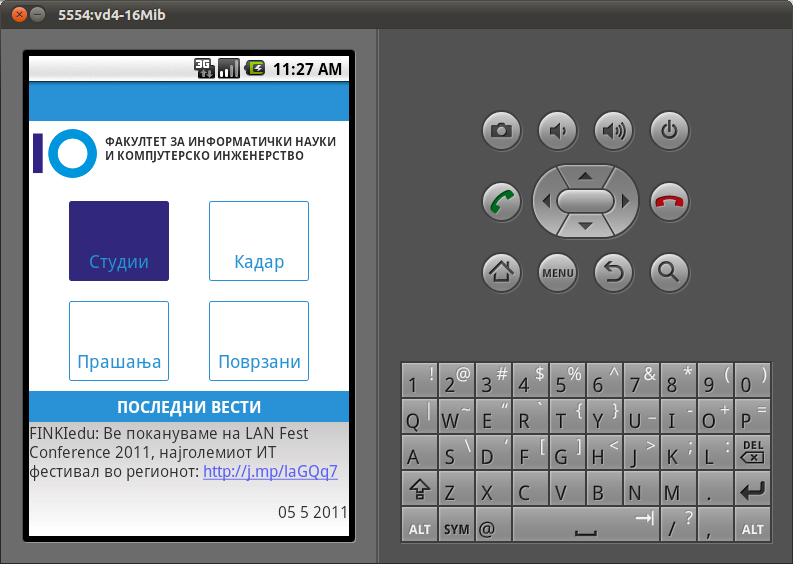
\includegraphics[scale=0.25]{images/emulator}
\end{center}
\end{frame}

\begin{frame}{Eclipse Plugin}
\begin{center}
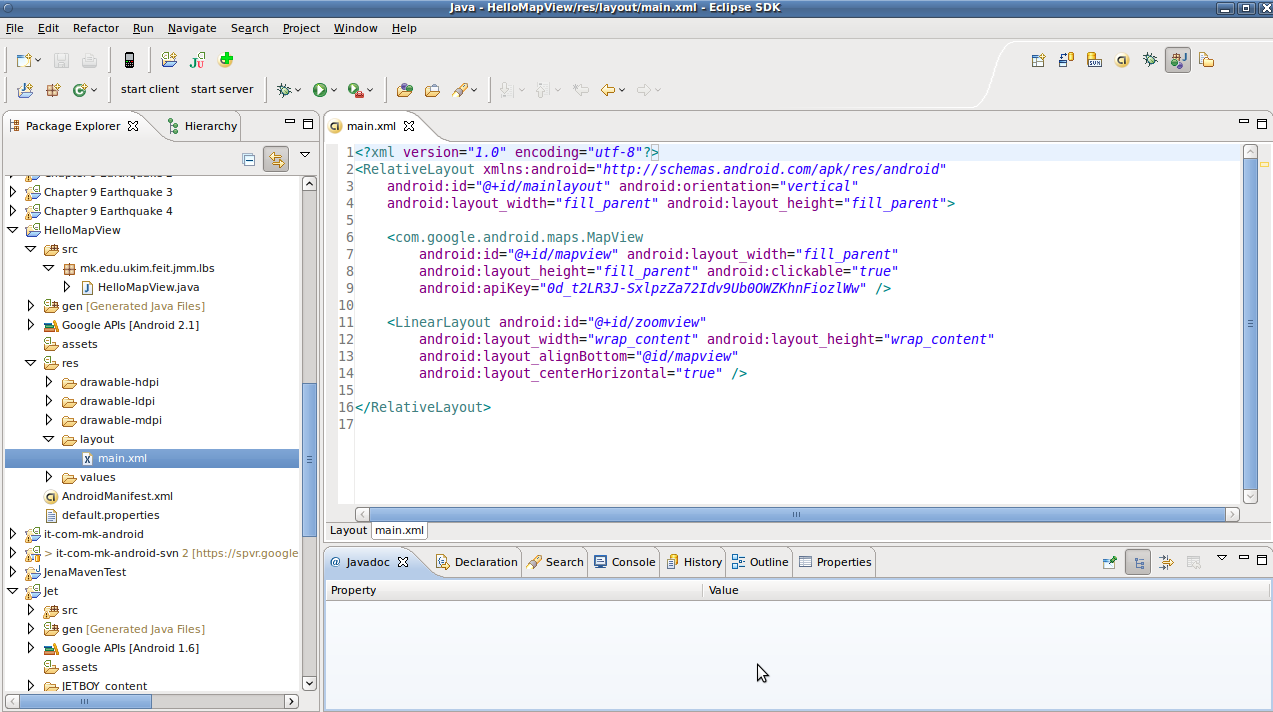
\includegraphics[scale=0.25]{images/eclipse}
\end{center}
\end{frame}

\begin{frame}{Dalvik Debug Monitor Server}
\begin{center}
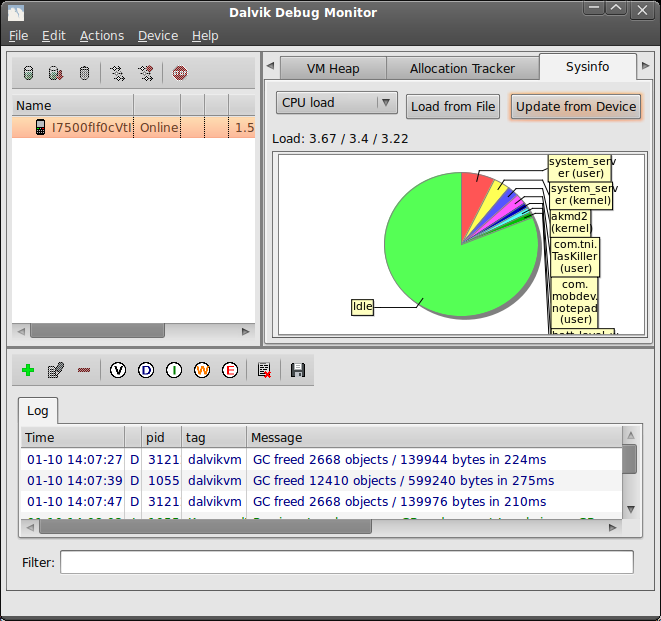
\includegraphics[scale=0.25]{images/ddms}
\end{center}
\end{frame}

\begin{frame}{Project Directory Layout}
\begin{center}
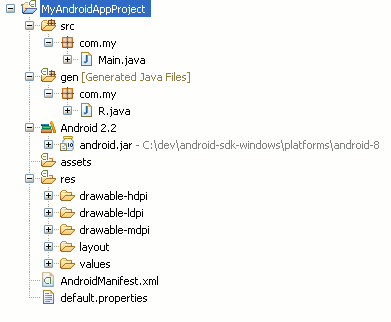
\includegraphics[scale=0.5]{images/project}
\end{center}
\end{frame}

\begin{frame}{Activity}
\begin{itemize}
    \item An Activity is an application component that
provides a screen with which users can
interact.
    \item Each activity is given a window in which to
draw its user interface.
    \item Typically, one activity in an application is
specified as the "\textbf{main}" activity, which is
presented to the user when launching the
application for the first time 
\end{itemize}
\end{frame}

\begin{frame}{Creating an Activity}{Part 1}
\begin{itemize}
    \item To create an activity, you must create a subclass of
\textbf{Activity}.
    \item In your subclass, you need to implement \textbf{callback
methods} that the system calls when the activity
transitions between various states of its lifecycle, such
as when the activity is being \textbf{created, stopped, resumed},
or \textbf{destroyed}.
\end{itemize}
\end{frame}

\begin{frame}{Creating an Activity}{Part 2}
\begin{itemize}
    \item \textbf{\texttt{onCreate()}}
    \begin{itemize}
        \item The system calls this when creating your activity. Within
your implementation, you should initialize the essential
components of your activity.
        \item Most importantly, this is where you must call setContentView() to
        define the layout for the activity's user interface.
    \end{itemize}
    \item \textbf{\texttt{onPause()}}
    \begin{itemize}
        \item The system calls this method as the first indication
that the user is leaving your activity.
        \item This is usually where you should commit any
changes that should be persisted beyond the current user session (because the
user might not come back).
    \end{itemize}     
\end{itemize}
\end{frame}

\begin{frame}{Implementing a user interface}{Views and widgets}
\begin{itemize}
  \item The user interface for an activity is provided by a hierarchy of
  views—objects derived from the View class.
  \item Each view controls a particular rectangular space within the activity's
  window and can respond to user interaction.
  \item For example, a view might be a button that initiates an action when the
  user touches it.
  \item "Widgets" are views that provide a visual (and interactive) elements for the screen, such as a button, text field, 
checkbox, or just an image. 
\end{itemize}
\end{frame} 

\begin{frame}{Implementing a user interface}{Layouts}
\begin{itemize}
  \item "Layouts" are views derived from ViewGroup that provide a unique layout model for its child views, 
such as a linear layout, a grid layout, or relative layout.
\begin{itemize} 
\item The most common way to define a layout using views is with an XML layout
file saved in your application resources.
\item This way, you can maintain the design of your user interface separately from the source code that defines the activity's behavior.
\item You can set the layout as the UI for your activity with setContentView(),
passing the resource ID for the layout.
\end{itemize}
\item You can also create new Views in your activity code and build a view
hierarchy by inserting new Views into a ViewGroup, then use that layout by passing the root ViewGroup to setContentView().
\end{itemize}
\end{frame}

\begin{frame}[fragile]{Declaring the activity in the manifest}
You must declare your activity in the manifest file in order for it to be
accessible to the system. To decalare your activity, 
open your manifest file and add an \texttt{<activity>} element as a child of
the \texttt{<application>} element.
\begin{exampleblock}{Example}
\begin{lstlisting}
<manifest ... >
  <application ... >
    <activity android:name=".ExampleActivity" />
        ...
  </application ... >
  ...
</manifest>
\end{lstlisting}
\end{exampleblock}
\end{frame}

\begin{frame}[fragile]{Using intent filters}
An \texttt{<activity>} element can also specify various intent filters—using the
\texttt{<intent-filter>} element—in order to declare how other application components may activate it.
\begin{exampleblock}{Example}
\begin{lstlisting}
<activity android:name=".ExampleActivity" android:icon="@drawable/app_icon">
    <intent-filter>
        <action android:name="android.intent.action.MAIN" />
        <category android:name="android.intent.category.LAUNCHER" />
    </intent-filter>
</activity>
\end{lstlisting}
\end{exampleblock}
\end{frame}

\begin{frame}[fragile]{Starting an Activity}
You can start another activity by calling \textbf{\texttt{startActivity()}}, passing it an 
\textbf{\texttt{Intent}} that describes the activity you want to start
\begin{exampleblock}{Example}
\begin{lstlisting}
Intent intent = new Intent(this, SignInActivity.class);
startActivity(intent);
\end{lstlisting}
\end{exampleblock}
\end{frame}


\begin{frame}{Shutting Down an Activity}
You can shut down an activity by calling its \textbf{\texttt{finish()}} method.
\\\vfill
You can also shut down a separate activity that you previously started by
calling \textbf{\texttt{finishActivity()}}.
\end{frame}

\begin{frame}{Implementing the lifecycle callbacks}
\begin{itemize}
  \item \texttt{onCreate}
  \item \texttt{onStart}
  \item \texttt{onResume}
  \item \texttt{onPause}
  \item \texttt{onStop}
  \item \texttt{onDestroy}
\end{itemize}
\end{frame}

\section{Android UI Part 1}
\begin{frame}{Activating components: intents}
\begin{itemize}
  \item Activities, services, and broadcast receivers are activated by
  asynchronous messages called \textbf{intents}
  \item An intent is an \texttt{Intent} object that holds the content of the
  message
\end{itemize}
\end{frame}

\begin{frame}{Fundamental Aandroid UI Design}
\begin{itemize}
  \item Views
  \begin{itemize}
  \item Views are the base class for all visual interface elements
  \item Derived from the View class
  \end{itemize}
  \item View Groups
  \begin{itemize}
  \item Can contain multiple child Views
  \item Extend the ViewGroup class
  \end{itemize}
  \item Activities
  \begin{itemize}
  \item Represent the window, or screen, being displayed.
  \item To display a user interface you assign a View (usually a layout) to an Activity
  \end{itemize}
\end{itemize}
\end{frame}

\begin{frame}[fragile]{Introducing Views}
\begin{exampleblock}{Inflating an Activity layout}
\begin{lstlisting}
@Override
public void onCreate(Bundle bundle) {
    super.onCreate(bundle);
    setContentView(R.layout.main);
    TextView textView = (TextView)findViewById(R.id.textView);
}
\end{lstlisting}
\end{exampleblock}
\begin{exampleblock}{Creating a UI layout in code}
\begin{lstlisting}
@Override
public void onCreate(Bundle bundle) {
    super.onCreate(bundle);
    TextView textView = new TextView(this);
    setContentView(textView);
    textView.setText("Hello Android");
}
\end{lstlisting}
\end{exampleblock}
\end{frame}

\begin{frame}{Event Listeners}
\begin{itemize}
  \item Java event handling mechanism
  \item Interfaces containing method that is invoked on some user action
  \item Examples Listeners:
  \begin{itemize}
  \item View.OnClickListener
  \item onClick(View v)
  \item View.OnKeyListener
  \item onKey(View v, int keyCode, KeyEvent event)
  \item View.OnTouchListener
  \item onTouch(View v, MotionEvent event)
  \end{itemize}
\end{itemize}
\end{frame}

\begin{frame}[fragile,shrink=20]{Using event listeners}
\begin{exampleblock}{Anonimous implementation of \texttt{OnClickListener}}
\begin{lstlisting}
private OnClickListener btnClicked = new OnClickListener() {
    public void onClick(View v) {
        // do something when button is clicked
    }
};
protected void onCreate(Bundle bundle) {
    // Capture our button from layout
    Button btn = (Button) findViewById(R.id.btn);
    // Register the onClick listener with the implementation above
    btn.setOnClickListener(btnClicked);
}
\end{lstlisting}
\end{exampleblock}
\begin{exampleblock}{In \texttt{XML}}
\begin{lstlisting}
<Button
    android:layout_width="wrap_content"
    android:layout_height="wrap_content"
    android:id="@+id/btnNewGame"
    android:onClick="onBtnClick"
    
public void onBtnClick(View view) {
    // do something when button is clicked
}
\end{lstlisting}
\end{exampleblock}
\end{frame}

\begin{frame}{Menus}
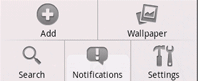
\includegraphics[scale=0.5]{images/menu}
\begin{itemize}
  \item Options Menu
  \begin{itemize}
  \item This is the primary set of menu items for an Activity
  \item It is revealed by pressing the device MENU key
  \end{itemize}
  \item Context Menu
  \begin{itemize}
  \item This is a floating list of menu items that may appear
when you perform a long-press on a View
  \end{itemize}
  \item Submenu
  \begin{itemize}
  \item This is a floating list of menu items that is revealed by
an item in the Options Menu or a Context Menu
  \end{itemize}
\end{itemize}
\end{frame}

\begin{frame}[fragile,shrink=10]{Options Menu}
When the menu is opened for the first time, the Android system will
call the Activity \texttt{onCreateOptionsMenu()} callback method
\begin{exampleblock}{The menu xml}
\begin{lstlisting}
<?xml version="1.0" encoding="utf-8"?>
<menu xmlns:android="http://schemas.android.com/apk/res/android">
    <item android:id="@+id/save_game" 
        android:title="@string/menu_save_game" />
    <item android:id="@+id/end_game" 
        android:title="@string/menu_end_game" />
</menu>
\end{lstlisting}
\end{exampleblock}
\begin{exampleblock}{Inflating the menu}
\begin{lstlisting}
@Override
public boolean onCreateOptionsMenu(Menu menu) {
    MenuInflater inflater = getMenuInflater();
    inflater.inflate(R.menu.game_menu, menu);
    return true;
}
\end{lstlisting}
\end{exampleblock}
\end{frame}

\section*{}

